\documentclass{article}
\usepackage{caption}
\usepackage{subcaption}
\usepackage{graphicx}
\usepackage{tikz}
\usepackage{tikzsymbols}
\usetikzlibrary{calc,patterns,shapes.geometric}
\usepackage{float}

\def\centerarc[#1](#2)(#3:#4:#5){\draw[#1] ($(#2)+({#5*cos(#3)},{#5*sin(#3)})$) arc (#3:#4:#5);}

\pagestyle{empty}
\begin{document}
	\centering
	\begin{figure}[H]
		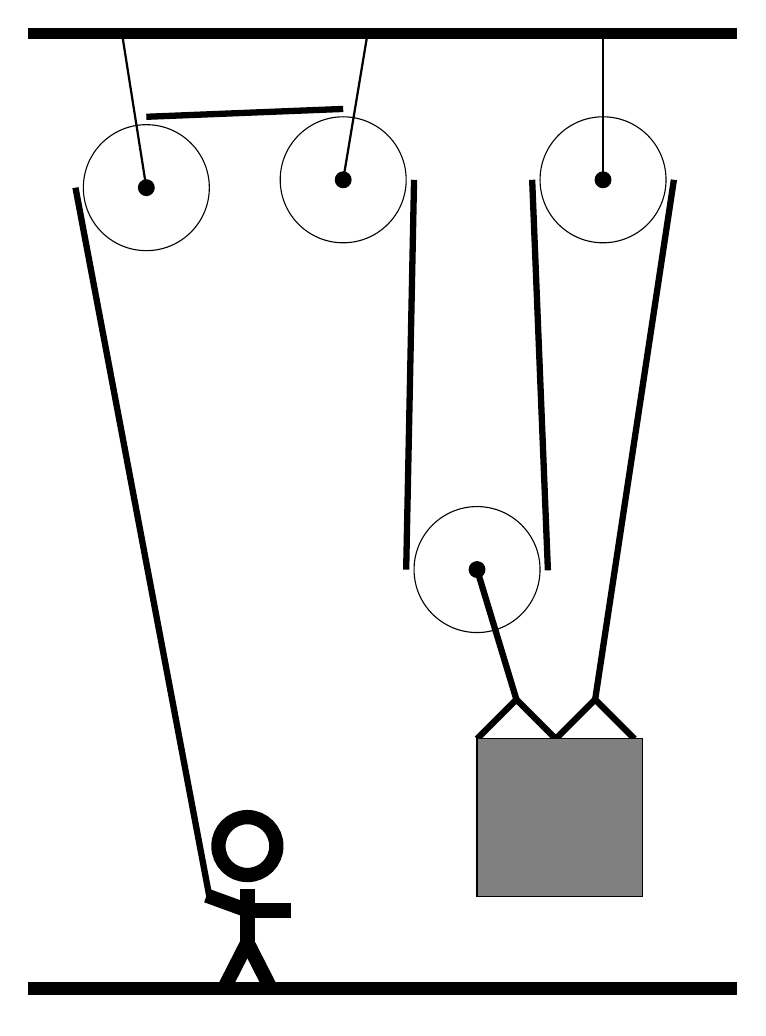
\begin{tikzpicture}
			%%%%% START %%%%%
			\def\a{9}
			\def\radlg{0.8}
			\def\radrp{0.9}
			\def\radsm{0.1}
			\def\xone{1}
			\def\yone{\a-0.2*\a}
			\def\xtwo{\xone+3.3}
			\def\ytwo{\a-0.2*\a}
			\def\xthree{\xone+1.7}
			\def\ythree{\a-0.75*\a}
			\def\xh{3.2}
			\def\hlen{\a+0.1}
			\def\width{0.8mm}
			\def\ywallone{\yone-0.1}
			\def\xwallone{\xone-2.5}
			\def\bump{0.3}
			
			\draw[fill=black] (-3,\a) rectangle (6,\a+0.125);
			
			\draw (\xone,\yone) circle (\radlg);
			\draw[fill=black] (\xone,\yone) circle (\radsm);
			\draw[thick] (\xone,\yone) -- (\xone+0.3,\a);
			
			\draw (\xtwo,\ytwo) circle (\radlg);
			\draw[fill=black] (\xtwo,\ytwo) circle (\radsm);
			\draw[thick] (\xtwo,\ytwo) -- (\xtwo,\a);
			
			\draw (\xthree,\ythree) circle (\radlg);
			\draw[fill=black] (\xthree,\ythree) circle (\radsm);
			
			\draw[line width=\width]  (\xh-0.5,\a-\hlen) -- (\xh,\a-\hlen+0.5) -- (\xh+0.5,\a-\hlen) -- (\xh+1,\a-\hlen+0.5) -- (\xh+1.5,\a-\hlen);
			\draw[fill=black!50] (\xh-0.5,\a-\hlen) rectangle (\xh+1.6,\a-\hlen-2);			
			
			\draw (\xwallone,\ywallone) circle (\radlg);
			\draw[fill=black] (\xwallone,\ywallone) circle (\radsm);
			\draw[thick] (\xwallone,\ywallone) -- (\xwallone-0.3,\a);
			
			\draw[line width=\width](-0.7,-1.9) -- 	 (\xwallone-\radrp, \ywallone);
			\centerarc[line width=\width](\xwallone,\ywallone)(90:180:\radrp);
			\draw[line width=\width](\xwallone, \ywallone+\radrp) -- (\xone,\yone+\radrp);
			\centerarc[line width=\width](\xone,\yone)(0:90:\radrp);
			\draw[line width=\width](\xone+\radrp,\yone) -- (\xthree-\radrp,\ythree);
			\centerarc[line width=\width](\xthree,\ythree)(180:370:\radrp);
			\draw[line width=\width] (\xthree+\radrp,\ythree-0.01) -- (\xtwo-\radrp,\ytwo);
			\centerarc[line width=\width](\xtwo,\ytwo)(0:180:\radrp);
			\draw[line width=\width](\xh+1,\a-\hlen+0.5) -- (\xtwo+\radrp,\ytwo);
			\draw[line width=\width] (\xh,\a-\hlen+0.5) -- (\xthree,\ythree);
			
			\node at (-0.2,-2) {\Strichmaxerl[10][-20][0]};
			
			\draw[fill=black] (-3,-3) rectangle (6,-3.15);
			%%%%% START %%%%%
		\end{tikzpicture}
	\end{figure}
	
\end{document}